\newpage
\appendix
\section{符号说明}
\label{sec:appendix-symbol}
\begin{table}[H]
    \centering
    \begin{tabularx}{0.95\textwidth}{>{\centering\arraybackslash}X>{\centering\arraybackslash}X>{\centering\arraybackslash}X}\toprule
        符号 & 含义 & 注释\\\midrule
        $\boldsymbol{x}_i$ & 特征向量 & \\\midrule
        $\boldsymbol{y}_i$ & 目标向量 & \\\midrule
        $\mathcal{X}$ & 特征向量集 & $\forall i:\boldsymbol{x}_i\in \mathcal{X}$ \\\midrule
        $\mathcal{Y}$ & 目标向量集 & $\forall i:\boldsymbol{y}_i\in \mathcal{Y}$ \\\midrule
        $D_{\text{tr}}$ & 训练集 & $D_{\text{tr}}={\{(\boldsymbol{x}_i, \boldsymbol{y}_i)\}}_{i=1}^{n}$\\\midrule
        $(\boldsymbol{x}_i, \boldsymbol{y}_i)$ & 单个样本 & $\boldsymbol{x}_i\in \mathcal{X}, y_i\in \mathcal{Y}$ \\\midrule 
        $P$ & 概率分布 & $(\boldsymbol{x}_i, \boldsymbol{y}_i)\sim P$ \\\midrule
        $f$ & 模型 & $f:\mathcal{X}\rightarrow \mathcal{Y}$ \\\midrule
        $\ell$ & 损失函数 &  \\\midrule
        $\|\cdot\|$ & 模长 &  \\\midrule
        $\mathcal{T}$ & 任务描述符序列 &  \\\midrule
        $(\boldsymbol{x}_i, t_i, \boldsymbol{y}_i)$ & 数据序列 & $\boldsymbol{x}_i\in \mathcal{X}, t_i\in \mathcal{T},y_i\in \mathcal{Y}$ \\\midrule
        $\left\langle\cdot,\cdot\right\rangle$ & 内积 &  \\\midrule
        $\nabla\cdot$ & 梯度算子 & $\nabla_\theta f=\frac{\partial f}{\partial\theta}$ \\\bottomrule
    \end{tabularx}
    \caption{符号说明}\label{tab:appendix-symbol}
\end{table}

\section{代码说明}
\subsection{\texorpdfstring{\lstinline{git diff}}{git diff}}
在终端运行 \lstinline{git diff main..raw --stat}, 可以展示我们对LibContinual进行的修改统计数据.
\lstinputlisting[language=bash]{codes/diff.txt}

\subsection{log file}
\label{sec:appendix-log}
下面展示了我们的日志, 由于我们的可视化输出使用的是 \lstinline{tqdm}, 因此进度条本身没有被记录在日志中, 只有结果保留在日志中了. 日志的部分截图如图~\ref{fig:log}~所示
\begin{figure}[H]
    \centering
    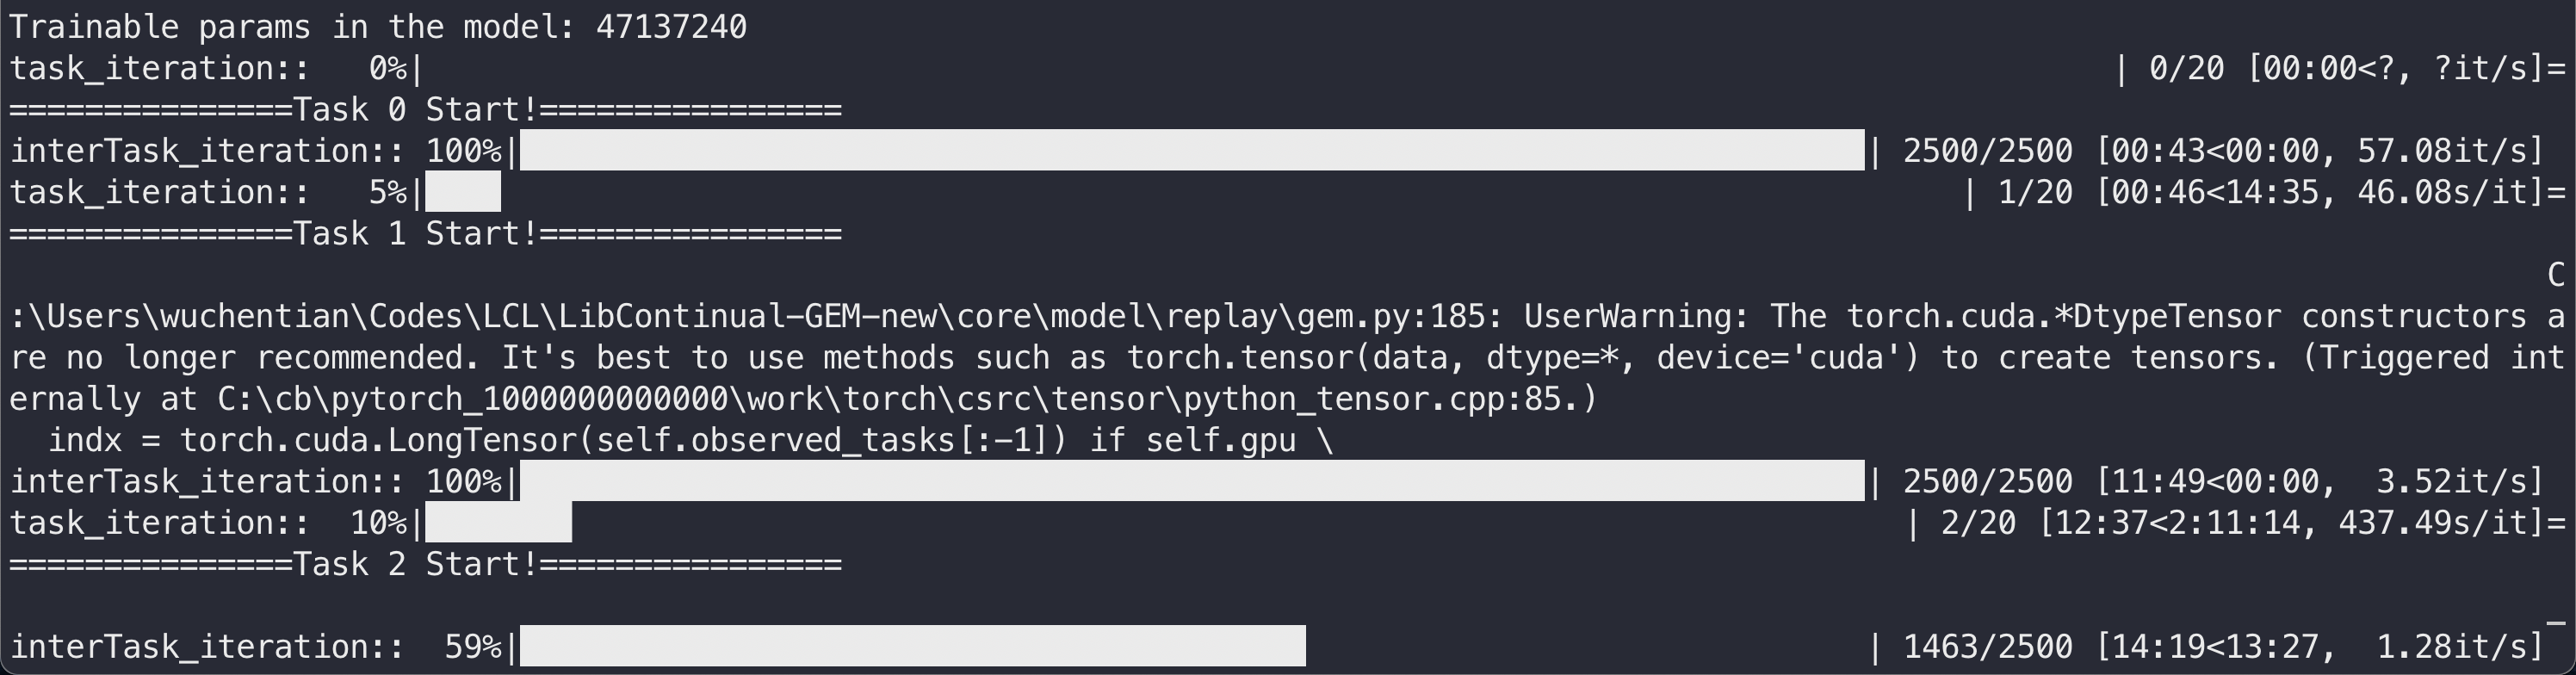
\includegraphics[width=1\linewidth]{log.png}
    \caption{日志部分截图}
    \label{fig:log}
\end{figure}
\lstinputlisting{codes/log.txt}